% introduction
\begin{frame}{Beamer}

    \begin{itemize}
        \item A beamer is one of the 10 \LaTeX  document classes.
        \item Beamer is used heavily for making great looking and standardized
            presentations (Eg: CambridgeUS theme)
        \item They can be simple like this one, but are also highly customizable
            like the one shown below
        \item The best part is, they are in PDF format.
    \end{itemize}

    \center
    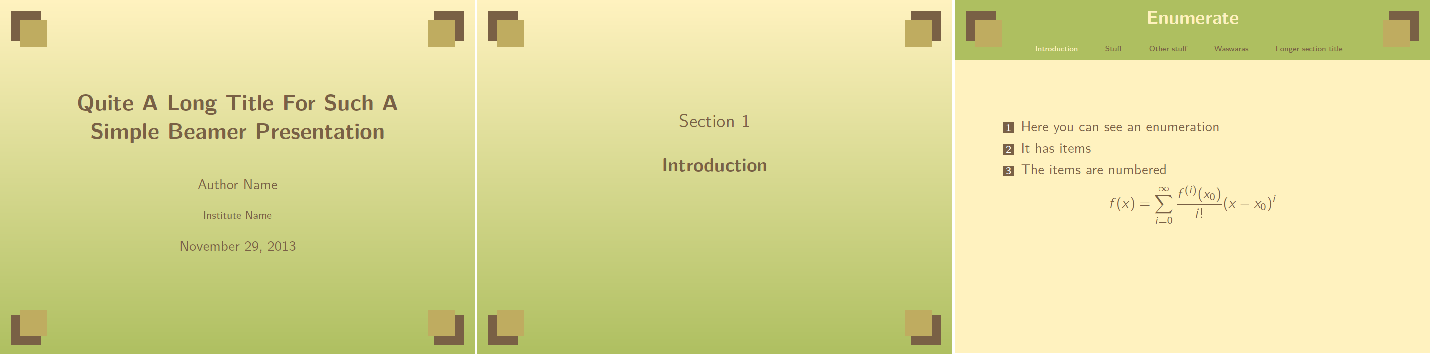
\includegraphics[width=\textwidth]{ugly.png}

\end{frame}

% Task
\begin{frame}{Beamer}{Task-1}
    Try solving the task-1.The solution is... \\ \pause
    \vspace{1em}
    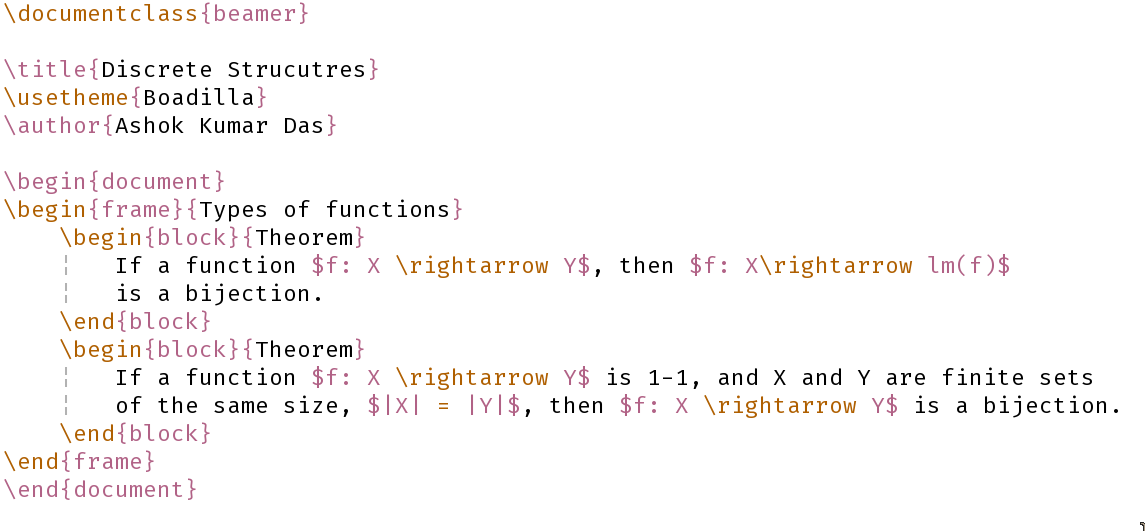
\includegraphics[width=\textwidth]{1.png}
\end{frame}
